% compile with $ pdflatex project_plan
\documentclass{article}
\usepackage[margin=1in]{geometry}
\usepackage{fancyhdr}
\usepackage{graphicx}
\usepackage{vhistory}
\usepackage[parfill]{parskip}
\graphicspath{{./}}

% Set fancy looking header/footer and move page number to the right
\pagestyle{fancy}
\fancyhead{}
\fancyfoot{}
\fancyfoot[R]{\thepage}

\title{}
\author{}
\date{}

\begin{document}

    \pagenumbering{gobble}
    \begin{titlepage}
    \begin{center}
        \vspace*{1cm}

        \Huge
        \textbf{User's Guide for Cloud Backup}

        \vspace{.5cm}
        \LARGE
        Captain CyBeard: Neil Before Us

        \vspace{1cm}

        \textbf{Ryan Breitenfeldt \textbar\ Noah Farris\\ Trevor Surface \textbar\ Kyle Thomas}

        \vspace{.2cm}
        \Large
        May 4, 2020

        \vspace{2cm}
        
\includegraphics[scale=1]{logo}

        \vfill

        Washington State University Tri-Cities\\
        CptS 423 Software Design Project 2

    \end{center}
\end{titlepage}



    \tableofcontents
    \listoffigures

    \newpage
    \begin{versionhistory}
        \vhEntry{0.4}{09.26.2019}{KT}{Filled in Approach section}
        \vhEntry{0.3}{09.24.2019}{RB NF TS KT}{Filled in scope and added diagram}
        \vhEntry{0.2}{09.19.2019}{KT}{Filled in Introduction Section}
        \vhEntry{0.1}{09.12.2019}{KT}{Document Creation}
    \end{versionhistory}
    \newpage

    \pagenumbering{arabic}

    \section{Introduction}
    This document is a project plan for developing a Django Web Application that allows Cypher Path users to enter
    a URL for online Virtual Machines and select which Virtual Machines will be downloaded onto Cypher Path's 
    servers. The purpose of the project plan is to provide a roadmap for Cypher Path and the software development
    team of the development process and help keep track of the progress.

    Subsequent sections of this project plan will cover the scope of the project, the software engineering
    approach that will be used for the project and an estimate for how long the project will take broken by task
    in the form of a Gantt Chart.

    \section{Scope}
    The project is to develop a Python-Django web application that allows a user that is logged into the application to enter a URL that points to one of several
    possible cloud based VM platforms and be presented with the authentication for that platform. After the user enters their credentials for the VM platform 
    they will be presented with the VM's they have on their account that are available to download.
    
    The application will present relevant information to the user such as the directory structure, names of the VM images, and a way to select which files and folders
    to download to their local machine.

    The first platform to focus on for interacting with will be VMware. Time permitting, other platforms such as Amazon Web Services (AWS), Citrix, Google Drive and Dropbox
    will be added. The application will have a modular design so other platforms can be added in the future.

    \begin{figure}[h]
    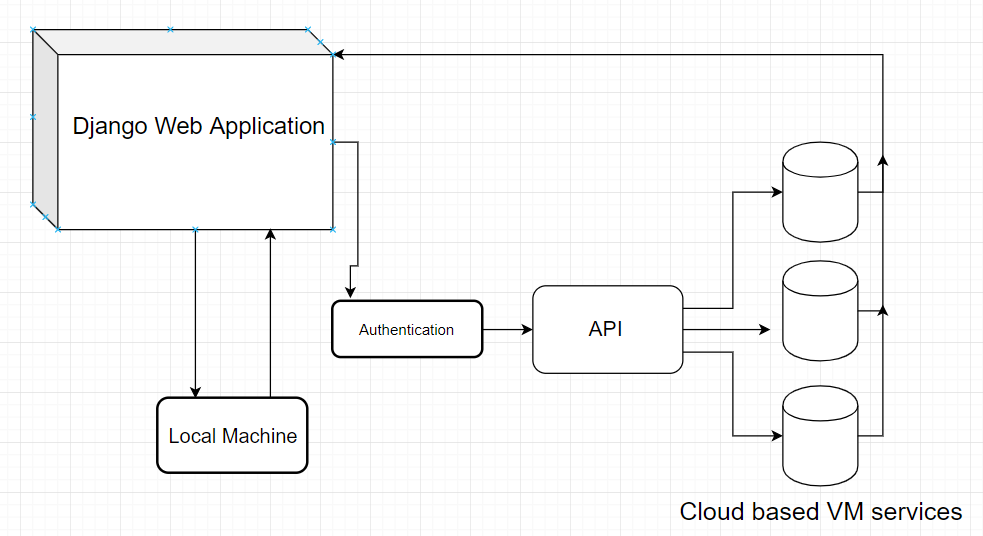
\includegraphics[scale=.7]{diagram}
        \caption{The application environment}
    \end{figure}

    \pagebreak
    \section{Approach}
    The software engineering approach that will be used for this project is the \textbf{Agile Scrum} approach.
    This iterative approach will ensure that the software development team will remain on track and that Cipherpath will receive the maximum amount of value
    for their time.

    The project will be implemented as a Python-Django web application, Python version 3+ and Django version 2+ will be used. The Python-Django framework provides the tools 
    and environment needed to develop and test a web application such as a lightweight web server and SQLite. For version control the software development team will be using git
    with a remote repository hosted on Github.

    \section{Estimate}

%    \section{References}
%
%    \appendix
%    \section{Appendix}

\end{document}
